% Generated by Sphinx.
\def\sphinxdocclass{report}
\documentclass[letterpaper,10pt,english]{sphinxmanual}
\usepackage[utf8]{inputenc}
\DeclareUnicodeCharacter{00A0}{\nobreakspace}
\usepackage{cmap}
\usepackage[T1]{fontenc}
\usepackage{babel}
\usepackage{times}
\usepackage[Bjarne]{fncychap}
\usepackage{longtable}
\usepackage{sphinx}
\usepackage{multirow}


\title{fantastico Documentation}
\date{April 20, 2013}
\release{0.0.1-b36}
\author{Radu Viorel Cosnita}
\newcommand{\sphinxlogo}{}
\renewcommand{\releasename}{Release}
\makeindex

\makeatletter
\def\PYG@reset{\let\PYG@it=\relax \let\PYG@bf=\relax%
    \let\PYG@ul=\relax \let\PYG@tc=\relax%
    \let\PYG@bc=\relax \let\PYG@ff=\relax}
\def\PYG@tok#1{\csname PYG@tok@#1\endcsname}
\def\PYG@toks#1+{\ifx\relax#1\empty\else%
    \PYG@tok{#1}\expandafter\PYG@toks\fi}
\def\PYG@do#1{\PYG@bc{\PYG@tc{\PYG@ul{%
    \PYG@it{\PYG@bf{\PYG@ff{#1}}}}}}}
\def\PYG#1#2{\PYG@reset\PYG@toks#1+\relax+\PYG@do{#2}}

\expandafter\def\csname PYG@tok@gd\endcsname{\def\PYG@tc##1{\textcolor[rgb]{0.63,0.00,0.00}{##1}}}
\expandafter\def\csname PYG@tok@gu\endcsname{\let\PYG@bf=\textbf\def\PYG@tc##1{\textcolor[rgb]{0.50,0.00,0.50}{##1}}}
\expandafter\def\csname PYG@tok@gt\endcsname{\def\PYG@tc##1{\textcolor[rgb]{0.00,0.27,0.87}{##1}}}
\expandafter\def\csname PYG@tok@gs\endcsname{\let\PYG@bf=\textbf}
\expandafter\def\csname PYG@tok@gr\endcsname{\def\PYG@tc##1{\textcolor[rgb]{1.00,0.00,0.00}{##1}}}
\expandafter\def\csname PYG@tok@cm\endcsname{\let\PYG@it=\textit\def\PYG@tc##1{\textcolor[rgb]{0.25,0.50,0.56}{##1}}}
\expandafter\def\csname PYG@tok@vg\endcsname{\def\PYG@tc##1{\textcolor[rgb]{0.73,0.38,0.84}{##1}}}
\expandafter\def\csname PYG@tok@m\endcsname{\def\PYG@tc##1{\textcolor[rgb]{0.13,0.50,0.31}{##1}}}
\expandafter\def\csname PYG@tok@mh\endcsname{\def\PYG@tc##1{\textcolor[rgb]{0.13,0.50,0.31}{##1}}}
\expandafter\def\csname PYG@tok@cs\endcsname{\def\PYG@tc##1{\textcolor[rgb]{0.25,0.50,0.56}{##1}}\def\PYG@bc##1{\setlength{\fboxsep}{0pt}\colorbox[rgb]{1.00,0.94,0.94}{\strut ##1}}}
\expandafter\def\csname PYG@tok@ge\endcsname{\let\PYG@it=\textit}
\expandafter\def\csname PYG@tok@vc\endcsname{\def\PYG@tc##1{\textcolor[rgb]{0.73,0.38,0.84}{##1}}}
\expandafter\def\csname PYG@tok@il\endcsname{\def\PYG@tc##1{\textcolor[rgb]{0.13,0.50,0.31}{##1}}}
\expandafter\def\csname PYG@tok@go\endcsname{\def\PYG@tc##1{\textcolor[rgb]{0.20,0.20,0.20}{##1}}}
\expandafter\def\csname PYG@tok@cp\endcsname{\def\PYG@tc##1{\textcolor[rgb]{0.00,0.44,0.13}{##1}}}
\expandafter\def\csname PYG@tok@gi\endcsname{\def\PYG@tc##1{\textcolor[rgb]{0.00,0.63,0.00}{##1}}}
\expandafter\def\csname PYG@tok@gh\endcsname{\let\PYG@bf=\textbf\def\PYG@tc##1{\textcolor[rgb]{0.00,0.00,0.50}{##1}}}
\expandafter\def\csname PYG@tok@ni\endcsname{\let\PYG@bf=\textbf\def\PYG@tc##1{\textcolor[rgb]{0.84,0.33,0.22}{##1}}}
\expandafter\def\csname PYG@tok@nl\endcsname{\let\PYG@bf=\textbf\def\PYG@tc##1{\textcolor[rgb]{0.00,0.13,0.44}{##1}}}
\expandafter\def\csname PYG@tok@nn\endcsname{\let\PYG@bf=\textbf\def\PYG@tc##1{\textcolor[rgb]{0.05,0.52,0.71}{##1}}}
\expandafter\def\csname PYG@tok@no\endcsname{\def\PYG@tc##1{\textcolor[rgb]{0.38,0.68,0.84}{##1}}}
\expandafter\def\csname PYG@tok@na\endcsname{\def\PYG@tc##1{\textcolor[rgb]{0.25,0.44,0.63}{##1}}}
\expandafter\def\csname PYG@tok@nb\endcsname{\def\PYG@tc##1{\textcolor[rgb]{0.00,0.44,0.13}{##1}}}
\expandafter\def\csname PYG@tok@nc\endcsname{\let\PYG@bf=\textbf\def\PYG@tc##1{\textcolor[rgb]{0.05,0.52,0.71}{##1}}}
\expandafter\def\csname PYG@tok@nd\endcsname{\let\PYG@bf=\textbf\def\PYG@tc##1{\textcolor[rgb]{0.33,0.33,0.33}{##1}}}
\expandafter\def\csname PYG@tok@ne\endcsname{\def\PYG@tc##1{\textcolor[rgb]{0.00,0.44,0.13}{##1}}}
\expandafter\def\csname PYG@tok@nf\endcsname{\def\PYG@tc##1{\textcolor[rgb]{0.02,0.16,0.49}{##1}}}
\expandafter\def\csname PYG@tok@si\endcsname{\let\PYG@it=\textit\def\PYG@tc##1{\textcolor[rgb]{0.44,0.63,0.82}{##1}}}
\expandafter\def\csname PYG@tok@s2\endcsname{\def\PYG@tc##1{\textcolor[rgb]{0.25,0.44,0.63}{##1}}}
\expandafter\def\csname PYG@tok@vi\endcsname{\def\PYG@tc##1{\textcolor[rgb]{0.73,0.38,0.84}{##1}}}
\expandafter\def\csname PYG@tok@nt\endcsname{\let\PYG@bf=\textbf\def\PYG@tc##1{\textcolor[rgb]{0.02,0.16,0.45}{##1}}}
\expandafter\def\csname PYG@tok@nv\endcsname{\def\PYG@tc##1{\textcolor[rgb]{0.73,0.38,0.84}{##1}}}
\expandafter\def\csname PYG@tok@s1\endcsname{\def\PYG@tc##1{\textcolor[rgb]{0.25,0.44,0.63}{##1}}}
\expandafter\def\csname PYG@tok@gp\endcsname{\let\PYG@bf=\textbf\def\PYG@tc##1{\textcolor[rgb]{0.78,0.36,0.04}{##1}}}
\expandafter\def\csname PYG@tok@sh\endcsname{\def\PYG@tc##1{\textcolor[rgb]{0.25,0.44,0.63}{##1}}}
\expandafter\def\csname PYG@tok@ow\endcsname{\let\PYG@bf=\textbf\def\PYG@tc##1{\textcolor[rgb]{0.00,0.44,0.13}{##1}}}
\expandafter\def\csname PYG@tok@sx\endcsname{\def\PYG@tc##1{\textcolor[rgb]{0.78,0.36,0.04}{##1}}}
\expandafter\def\csname PYG@tok@bp\endcsname{\def\PYG@tc##1{\textcolor[rgb]{0.00,0.44,0.13}{##1}}}
\expandafter\def\csname PYG@tok@c1\endcsname{\let\PYG@it=\textit\def\PYG@tc##1{\textcolor[rgb]{0.25,0.50,0.56}{##1}}}
\expandafter\def\csname PYG@tok@kc\endcsname{\let\PYG@bf=\textbf\def\PYG@tc##1{\textcolor[rgb]{0.00,0.44,0.13}{##1}}}
\expandafter\def\csname PYG@tok@c\endcsname{\let\PYG@it=\textit\def\PYG@tc##1{\textcolor[rgb]{0.25,0.50,0.56}{##1}}}
\expandafter\def\csname PYG@tok@mf\endcsname{\def\PYG@tc##1{\textcolor[rgb]{0.13,0.50,0.31}{##1}}}
\expandafter\def\csname PYG@tok@err\endcsname{\def\PYG@bc##1{\setlength{\fboxsep}{0pt}\fcolorbox[rgb]{1.00,0.00,0.00}{1,1,1}{\strut ##1}}}
\expandafter\def\csname PYG@tok@kd\endcsname{\let\PYG@bf=\textbf\def\PYG@tc##1{\textcolor[rgb]{0.00,0.44,0.13}{##1}}}
\expandafter\def\csname PYG@tok@ss\endcsname{\def\PYG@tc##1{\textcolor[rgb]{0.32,0.47,0.09}{##1}}}
\expandafter\def\csname PYG@tok@sr\endcsname{\def\PYG@tc##1{\textcolor[rgb]{0.14,0.33,0.53}{##1}}}
\expandafter\def\csname PYG@tok@mo\endcsname{\def\PYG@tc##1{\textcolor[rgb]{0.13,0.50,0.31}{##1}}}
\expandafter\def\csname PYG@tok@mi\endcsname{\def\PYG@tc##1{\textcolor[rgb]{0.13,0.50,0.31}{##1}}}
\expandafter\def\csname PYG@tok@kn\endcsname{\let\PYG@bf=\textbf\def\PYG@tc##1{\textcolor[rgb]{0.00,0.44,0.13}{##1}}}
\expandafter\def\csname PYG@tok@o\endcsname{\def\PYG@tc##1{\textcolor[rgb]{0.40,0.40,0.40}{##1}}}
\expandafter\def\csname PYG@tok@kr\endcsname{\let\PYG@bf=\textbf\def\PYG@tc##1{\textcolor[rgb]{0.00,0.44,0.13}{##1}}}
\expandafter\def\csname PYG@tok@s\endcsname{\def\PYG@tc##1{\textcolor[rgb]{0.25,0.44,0.63}{##1}}}
\expandafter\def\csname PYG@tok@kp\endcsname{\def\PYG@tc##1{\textcolor[rgb]{0.00,0.44,0.13}{##1}}}
\expandafter\def\csname PYG@tok@w\endcsname{\def\PYG@tc##1{\textcolor[rgb]{0.73,0.73,0.73}{##1}}}
\expandafter\def\csname PYG@tok@kt\endcsname{\def\PYG@tc##1{\textcolor[rgb]{0.56,0.13,0.00}{##1}}}
\expandafter\def\csname PYG@tok@sc\endcsname{\def\PYG@tc##1{\textcolor[rgb]{0.25,0.44,0.63}{##1}}}
\expandafter\def\csname PYG@tok@sb\endcsname{\def\PYG@tc##1{\textcolor[rgb]{0.25,0.44,0.63}{##1}}}
\expandafter\def\csname PYG@tok@k\endcsname{\let\PYG@bf=\textbf\def\PYG@tc##1{\textcolor[rgb]{0.00,0.44,0.13}{##1}}}
\expandafter\def\csname PYG@tok@se\endcsname{\let\PYG@bf=\textbf\def\PYG@tc##1{\textcolor[rgb]{0.25,0.44,0.63}{##1}}}
\expandafter\def\csname PYG@tok@sd\endcsname{\let\PYG@it=\textit\def\PYG@tc##1{\textcolor[rgb]{0.25,0.44,0.63}{##1}}}

\def\PYGZbs{\char`\\}
\def\PYGZus{\char`\_}
\def\PYGZob{\char`\{}
\def\PYGZcb{\char`\}}
\def\PYGZca{\char`\^}
\def\PYGZam{\char`\&}
\def\PYGZlt{\char`\<}
\def\PYGZgt{\char`\>}
\def\PYGZsh{\char`\#}
\def\PYGZpc{\char`\%}
\def\PYGZdl{\char`\$}
\def\PYGZhy{\char`\-}
\def\PYGZsq{\char`\'}
\def\PYGZdq{\char`\"}
\def\PYGZti{\char`\~}
% for compatibility with earlier versions
\def\PYGZat{@}
\def\PYGZlb{[}
\def\PYGZrb{]}
\makeatother

\begin{document}

\maketitle
\tableofcontents
\phantomsection\label{index::doc}



\chapter{Introduction}
\label{intro:introduction}\label{intro::doc}\label{intro:fantastico-framework}

\section{Why another python framework?}
\label{intro:why-another-python-framework}
The main reason for developing a new framework is simple: I want to use it for teaching purposes. I have seen
many projects which fail either because of poor coding or because they become legacy very fast. I will not get into details
why and what could have been done. It defeats the purpose.

Each piece of code that is being added to fantastico will follow these simple rules:
\begin{enumerate}
\item {} 
\emph{The code is written because is needed and there is no clean way to achieve the requirement with existing fantastico features}.

\item {} 
The code is developed using TDD (Test Driven Development).

\item {} 
The code quality is 9+ (reported by pylint).

\item {} 
The code coverage is 90\%+ (reported by nose coverage).

\item {} 
The code is fully documented and included into documentation.

\end{enumerate}


\subsection{What do you want to teach who?}
\label{intro:what-do-you-want-to-teach-who}
I am a big fan of Agile practices and currently I own a domain called scrum-expert.ro. This is meant to become a collection of
hands on resource of how to develop good software with high quality and in a reasonable amount of time. Resources will cover topics
like
\begin{enumerate}
\item {} 
Incremental development always ready for rollout.

\item {} 
TDD (Test Driven Development)

\item {} 
XP (eXtreme programming)

\item {} 
Scrum

\item {} 
Projects setup for Continuous Delivery

\end{enumerate}

and many other topics that are required for delivering high quality software but apparently so many companies are ignoring nowadays.


\section{Fantastico's initial ideas}
\label{intro:fantastico-s-initial-ideas}\begin{itemize}
\item {} 
Very fast and pluggable routing engine.

\item {} 
Easily creation of REST apis.

\item {} 
Easily publishing of content (dynamic content).

\item {} 
Easily composition of available content.

\item {} 
Easily deployment on non expensive infrastructures (AWS, RackSpace).

\end{itemize}

Once the features above are developed there should be extremely easy to create the following sample applications:
\begin{enumerate}
\item {} 
Blog development

\item {} 
Web Forms development.

\item {} 
Personal web sites.

\end{enumerate}


\chapter{Getting started}
\label{get_started/getting_started:getting-started}\label{get_started/getting_started::doc}

\section{Installation manual}
\label{get_started/installation:installation-manual}\label{get_started/installation::doc}
In this section you can find out how to configure fantastico framework for different purposes.


\subsection{Developing a new fantastico project}
\label{get_started/installation:developing-a-new-fantastico-project}
Currently fantastico is in early stages so we did not really use it to create new projects. The desired way we want
to provide this is presented below:

pip-3.2 install fantastico

Done, now you are ready to follow our tutorials about creating new projects.


\subsection{Contributing to fantastico framework}
\label{get_started/installation:contributing-to-fantastico-framework}
Fantastico is an open source MIT licensed project to which any contribution is welcomed. If you like this framework idea
and you want to contribute do the following (I assume you are on an ubuntu machine):

\begin{Verbatim}[commandchars=\\\{\}]
\PYG{c}{\PYGZsh{}. Create a github account.}
\PYG{c}{\PYGZsh{}. Ask for permissions to contribute to this project (send an email to radu.cosnita@gmail.com) \PYGZhy{} I will gladly grant you permissions.}
\PYG{c}{\PYGZsh{}. Create a folder where you want to hold fantastico framework files. (e.g worspace\PYGZus{}fantastico)}
\PYG{c}{\PYGZsh{}. cd \PYGZti{}/workspace\PYGZus{}fantastico}
\PYG{c}{\PYGZsh{}. git clone git@github.com:rcosnita/fantastico}
\PYG{c}{\PYGZsh{}. sudo apt\PYGZhy{}get install python3\PYGZhy{}setuptools}
\PYG{c}{\PYGZsh{}. sh virtual\PYGZus{}env/setup\PYGZus{}dev\PYGZus{}env.sh}
\PYG{c}{\PYGZsh{}. cd \PYGZti{}/workspace\PYGZus{}fantastico}
\PYG{c}{\PYGZsh{}. git clone git@github.com:rcosnita/fantastico fantastico\PYGZhy{}doc}
\PYG{c}{\PYGZsh{}. git checkout gh\PYGZhy{}pages}
\end{Verbatim}

Now you have a fully functional fantastico workspace. I personally use PyDev and spring toolsuite but you are free to use
whatever editor you want. The only rule we follow is \emph{always keep the code stable}. To check the stability of your contribution
before commiting the code follow the steps below:

\begin{Verbatim}[commandchars=\\\{\}]
\PYG{c}{\PYGZsh{}. cd \PYGZti{}/workspace\PYGZus{}fantastico/fantastico/fantastico}
\PYG{c}{\PYGZsh{}. sh run\PYGZus{}tests.sh (we expect no failure in here)}
\PYG{c}{\PYGZsh{}. sh run\PYGZus{}pylint.sh (we expect 9+ rated code otherwise the build will fail).}
\PYG{c}{\PYGZsh{}. cd \PYGZti{}/workspace\PYGZus{}fantastico/fantastico}
\PYG{c}{\PYGZsh{}. export BUILD\PYGZus{}NUMBER=1}
\PYG{c}{\PYGZsh{}. ./build\PYGZus{}docs.sh (this will autogenerate documentation).}
\PYG{c}{\PYGZsh{}. Look into \PYGZti{}/workspace\PYGZus{}fantastico/fantastico\PYGZhy{}doc}
\PYG{c}{\PYGZsh{}. Here you can see the autogenerated documentation (do not commit this as Jenkins will do this for you).}
\PYG{c}{\PYGZsh{}. Be brave and push your newly awesome contribution.}
\end{Verbatim}


\section{Fantastico settings}
\label{get_started/settings:fantastico-settings}\label{get_started/settings::doc}
Fantastico is configured using a plain settings file. This file is located in the root of fantastico framework
or in the root folder of your project. Before we dig further into configuration options lets see a very simple settings
file:

\begin{Verbatim}[commandchars=\\\{\}]
\PYG{n}{installed\PYGZus{}middleware} \PYG{o}{=} \PYG{p}{[}\PYG{l+s}{\PYGZsq{}}\PYG{l+s}{fantastico.core.middleware.RequestResponseMiddleware}\PYG{l+s}{\PYGZsq{}}\PYG{p}{,}
                        \PYG{l+s}{\PYGZsq{}}\PYG{l+s}{fantastico.core.middleware.RoutingEngineMiddleware}\PYG{l+s}{\PYGZsq{}}\PYG{p}{]}
\end{Verbatim}

The above code sample represent the minimum required configuration for fantastico framework to run. The order in which
middlewares are listed is the order in which they are executed when an http request is made.


\subsection{Settings API}
\label{get_started/settings:settings-api}
Below you can find technical information about settings.
\index{BasicSettings (class in fantastico.settings)}

\begin{fulllineitems}
\phantomsection\label{get_started/settings:fantastico.settings.BasicSettings}\pysigline{\strong{class }\code{fantastico.settings.}\bfcode{BasicSettings}}
This is the core class that describes all available settings of fantastico framework. For convenience all options
have default values that ensure minimum functionality of the framework.

\end{fulllineitems}



\subsection{Create Dev configuration}
\label{get_started/settings:create-dev-configuration}

\subsection{Create Prod configuration}
\label{get_started/settings:create-prod-configuration}

\chapter{Fantastico features}
\label{features/features::doc}\label{features/features:fantastico-features}

\section{Request lifecycle}
\label{features/request_response:request-lifecycle}\label{features/request_response::doc}
In this document you can find how a request is processed by fantastico framework. By default WSGI applications use a dictionary
that contains various useful keys:
\begin{itemize}
\item {} 
HTTP Headers

\item {} 
HTTP Cookies

\item {} 
Helper keys (e.g file wrapper).

\end{itemize}

In fantastico we want to hide the complexity of this dictionary and allow developers to use some standardized objects. Fantastico
framework follows a Request / Response paradigm. This mean that for every single http request only one single http response will
be generated. Below, you can find a simple example of how requests are processed by fantastico framework:

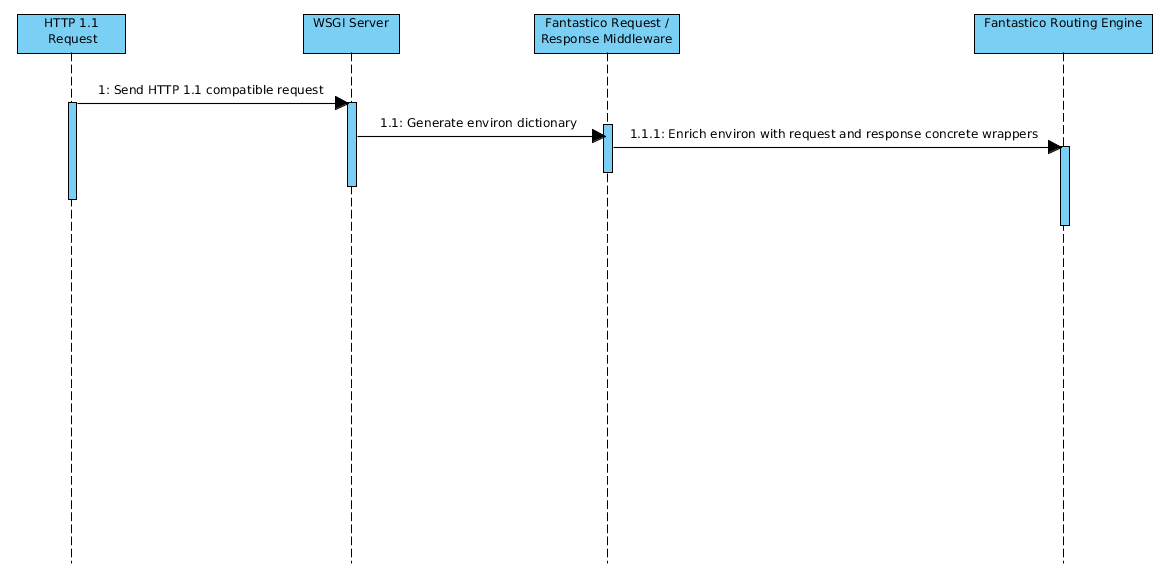
\includegraphics{request_response_sd.png}

In order to not reinvent the wheels fantastico relies on WebOb python framework in order to correctly generate request and response
objects. For more information read \href{http://docs.webob.org/en/latest/reference.html}{WebOB Doc}.


\section{Routing engine}
\label{features/routing_engine:routing-engine}\label{features/routing_engine::doc}
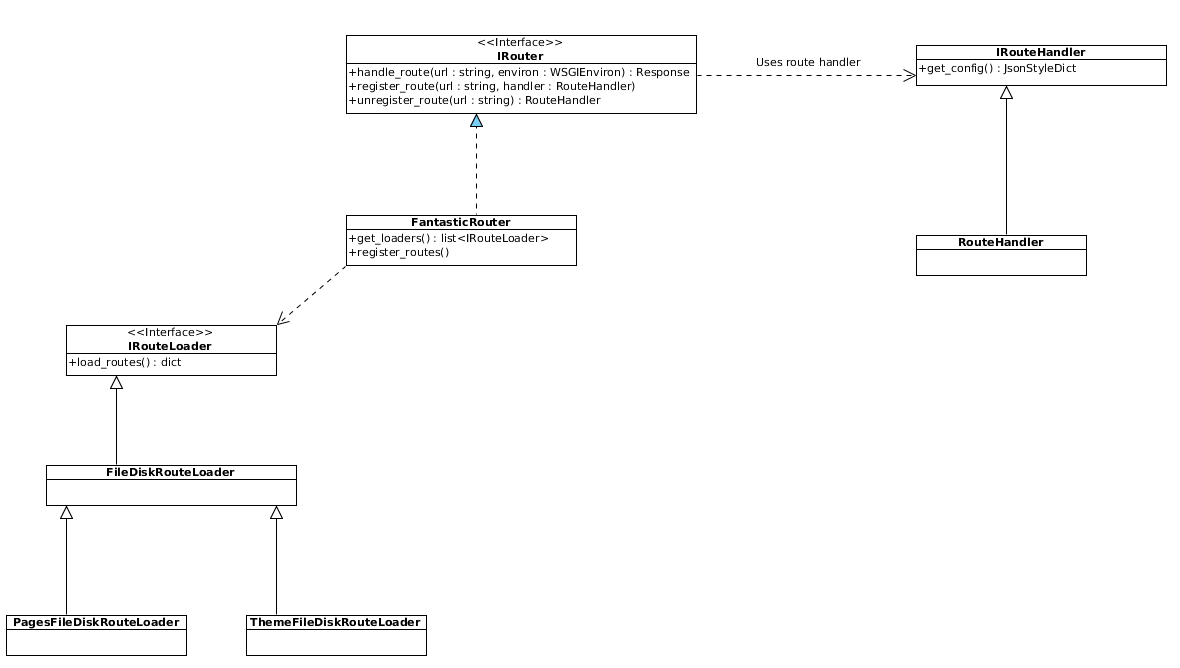
\includegraphics{routing_engine.png}


\chapter{Build status}
\label{index:build-status}
If you want to see the current build status of the project visit \href{http://jenkins.scrum-expert.ro:8080/job/fantastico-framework/badge/icon/}{Build status}.


\chapter{License}
\label{index:license}
Copyright 2013 Cosnita Radu Viorel

Permission is hereby granted, free of charge, to any person obtaining a copy of this software and associated
documentation files (the ``Software''), to deal in the Software without restriction, including without limitation
the rights to use, copy, modify, merge, publish, distribute, sublicense, and/or sell copies of the Software,
and to permit persons to whom the Software is furnished to do so, subject to the following conditions:

The above copyright notice and this permission notice shall be included in all copies or substantial portions of the Software.

THE SOFTWARE IS PROVIDED ``AS IS'', WITHOUT WARRANTY OF ANY KIND, EXPRESS OR IMPLIED, INCLUDING BUT NOT LIMITED TO THE
WARRANTIES OF MERCHANTABILITY, FITNESS FOR A PARTICULAR PURPOSE AND NONINFRINGEMENT. IN NO EVENT SHALL THE AUTHORS OR
COPYRIGHT HOLDERS BE LIABLE FOR ANY CLAIM, DAMAGES OR OTHER LIABILITY, WHETHER IN AN ACTION OF CONTRACT, TORT OR OTHERWISE,
ARISING FROM, OUT OF OR IN CONNECTION WITH THE SOFTWARE OR THE USE OR OTHER DEALINGS IN THE SOFTWARE.



\renewcommand{\indexname}{Index}
\printindex
\end{document}
